% Technical report. Build with:  python scripts/build_paper.py
% (or, from this directory:  tectonic paper.tex)
\documentclass[11pt]{article}

\usepackage[margin=1in]{geometry}
\usepackage{graphicx}
\usepackage{booktabs}
\usepackage{amsmath}
\usepackage{caption}
\usepackage{subcaption}
\usepackage[hidelinks]{hyperref}
\usepackage{xcolor}

\graphicspath{{figures/}}

\title{\textbf{Does masked pretraining learn the structure of mixed spectra?}\\
\large A controlled study on synthetic NMR-like mixtures with exact ground truth}
\author{Tanmay Hinge\\\small \texttt{hingetanmay@gmail.com}}
\date{\today}

\begin{document}
\maketitle

\begin{abstract}
\noindent
Self-supervised masked modeling is the standard recipe for pretraining sequence models, but
it is not obvious that hiding parts of a one-dimensional spectrum teaches a model anything
about the physical structure that generated it. I study this on synthetic mixtures of
NMR-like spectra, where every mixture is built from a known component library and therefore
ships with exact ground truth: which compounds are present, at what concentration, and each
component's clean signal. The main finding is that the answer depends on how you measure.
Judged by end-task accuracy after full fine-tuning, masked pretraining is worth almost
nothing, because the task is easy enough that a from-scratch model catches up. Judged by what
is \emph{linearly decodable} from the frozen representation, the same pretraining is worth a
great deal: presence macro-F1 rises from 0.729 to 0.872 over a random encoder, and
concentration error nearly matches a supervised encoder that never trained on concentration.
Sweeping a difficulty knob resolves the tension and exposes a sharper limitation: as the
signal-to-noise ratio falls from 40 to 6, the fine-tuning gain grows to $+0.082$ macro-F1 at
40 labels, yet the frozen self-supervised representation collapses to 0.529 presence macro-F1
while a supervised encoder still reaches 0.921 on the same data. The information survives the
noise; the pretext task stops capturing it. A target-swap ablation then refutes the obvious
explanation: handed a perfect noise-free reconstruction target - an oracle - the pretext
recovers only 2\% of that gap, so noise in the target is not the culprit, and the noise-robust
objectives one would reach for next are ruled out rather than indicated. All code, configs, and
seeds are public and the study reruns from one command.
\end{abstract}

\section{Introduction}

Mixture analysis appears whenever an instrument measures a sum of overlapping signals and we
want the parts back. Nuclear magnetic resonance (NMR) spectra in drug screening are a
concrete case: a measured spectrum superposes contributions from several compounds, and the
practical question is which compounds are present and in what amounts. Real screening data is
proprietary and, more importantly for a study like this one, does not come with a trustworthy
decomposition into ground-truth parts. Without that decomposition you can train a model but
you cannot cleanly measure whether a claimed separation is correct.

Synthetic data solves the measurement problem. If each mixture is built from known components,
the exact answer is available for every sample. The cost is realism, and I take that tradeoff
deliberately: the goal is not a chemistry-grade tool but a clean, reproducible study of a
method, run in miniature, where every claim can be checked against generated truth.

The method under test is masked sequence modeling: hide part of an input, ask the model to
reconstruct the hidden part, use no labels~\cite{bert,mae}. The hypothesis worth checking is
that applied to raw spectra it teaches a model where peaks sit, how wide they are, and how
they cluster into per-compound patterns, and that this structure transfers to the labeled
tasks that matter. The contributions are:

\begin{itemize}
  \item A synthetic mixture factory with an exact reconstruction identity and a single
        difficulty knob (Section~\ref{sec:data}).
  \item A controlled fine-tuning comparison showing masked pretraining is \emph{near-useless}
        on the easy regime at every label budget (Section~\ref{sec:finetune}).
  \item Frozen linear probes showing the \emph{same} representation is much better organized
        than a random one, which reframes that null result (Section~\ref{sec:probes}).
  \item A difficulty sweep showing the two measurements diverge as noise grows, and localizing
        the failure to the pretext objective rather than the task (Section~\ref{sec:robust}).
  \item An ablation that \emph{refutes} the natural explanation for that failure, closing off a
        plausible research direction rather than confirming one (Section~\ref{sec:ablation}).
\end{itemize}

\section{Synthetic data generation}
\label{sec:data}

Everything downstream is graded against the data factory, so correctness there was the
priority. A spectrum is a fixed grid of 2048 intensities over a 0--10~ppm axis, the usual
proton NMR range. The $\approx$0.005~ppm spacing resolves narrow peaks and their J-coupling
splitting, and the grid length is a power of two, which matters for patch tokenization later.

A component is a compound with a fixed pattern of peaks. I generate a library of 12 compounds
once from a fixed seed and freeze it to disk, so every experiment sees the same fingerprints.
Peak positions are drawn with priors placing them in realistic proton regions (aromatic
$\approx$6.5--8.5~ppm, an intermediate band, aliphatic $\approx$0.5--3~ppm). Each peak is
rendered as a Lorentzian, the physically correct lineshape for relaxation-limited NMR lines,
and peaks may split into multiplets by J-coupling with Pascal-triangle intensities so total
area is conserved. Fixing the library is what makes ``which compounds are present'' a
well-defined classification target rather than an ill-posed question about arbitrary peaks.
The library sits behind a small interface, so real single-compound spectra could be
substituted later without touching the rest of the pipeline.

A mixture chooses $K \in [2,5]$ compounds, assigns positive concentrations, sums the scaled
fingerprints, and applies corruptions standing in for instrument imperfections: additive
Gaussian noise at a target signal-to-noise ratio (SNR), a slow rolling baseline, and a small
random shift in peak positions. SNR follows the NMR convention, tallest peak height over noise
standard deviation. Position jitter is applied while rendering each component, so it lands
inside the stored ground-truth component signals. That detail keeps an exact identity intact:
\begin{equation}
  \text{mixture} = \sum_i \text{clean component}_i + \text{baseline} + \text{noise}.
  \label{eq:identity}
\end{equation}
Equation~\ref{eq:identity} holds to zero floating-point error, and a test checks it on every
generated sample. Each mixture ships with a multi-hot presence vector, a concentration vector,
and the clean per-component signals. Samples are generated on demand from a seed and an index
rather than stored, so any sample is reproducible and no dataset is ever written to disk.

\begin{figure}[t]
  \centering
  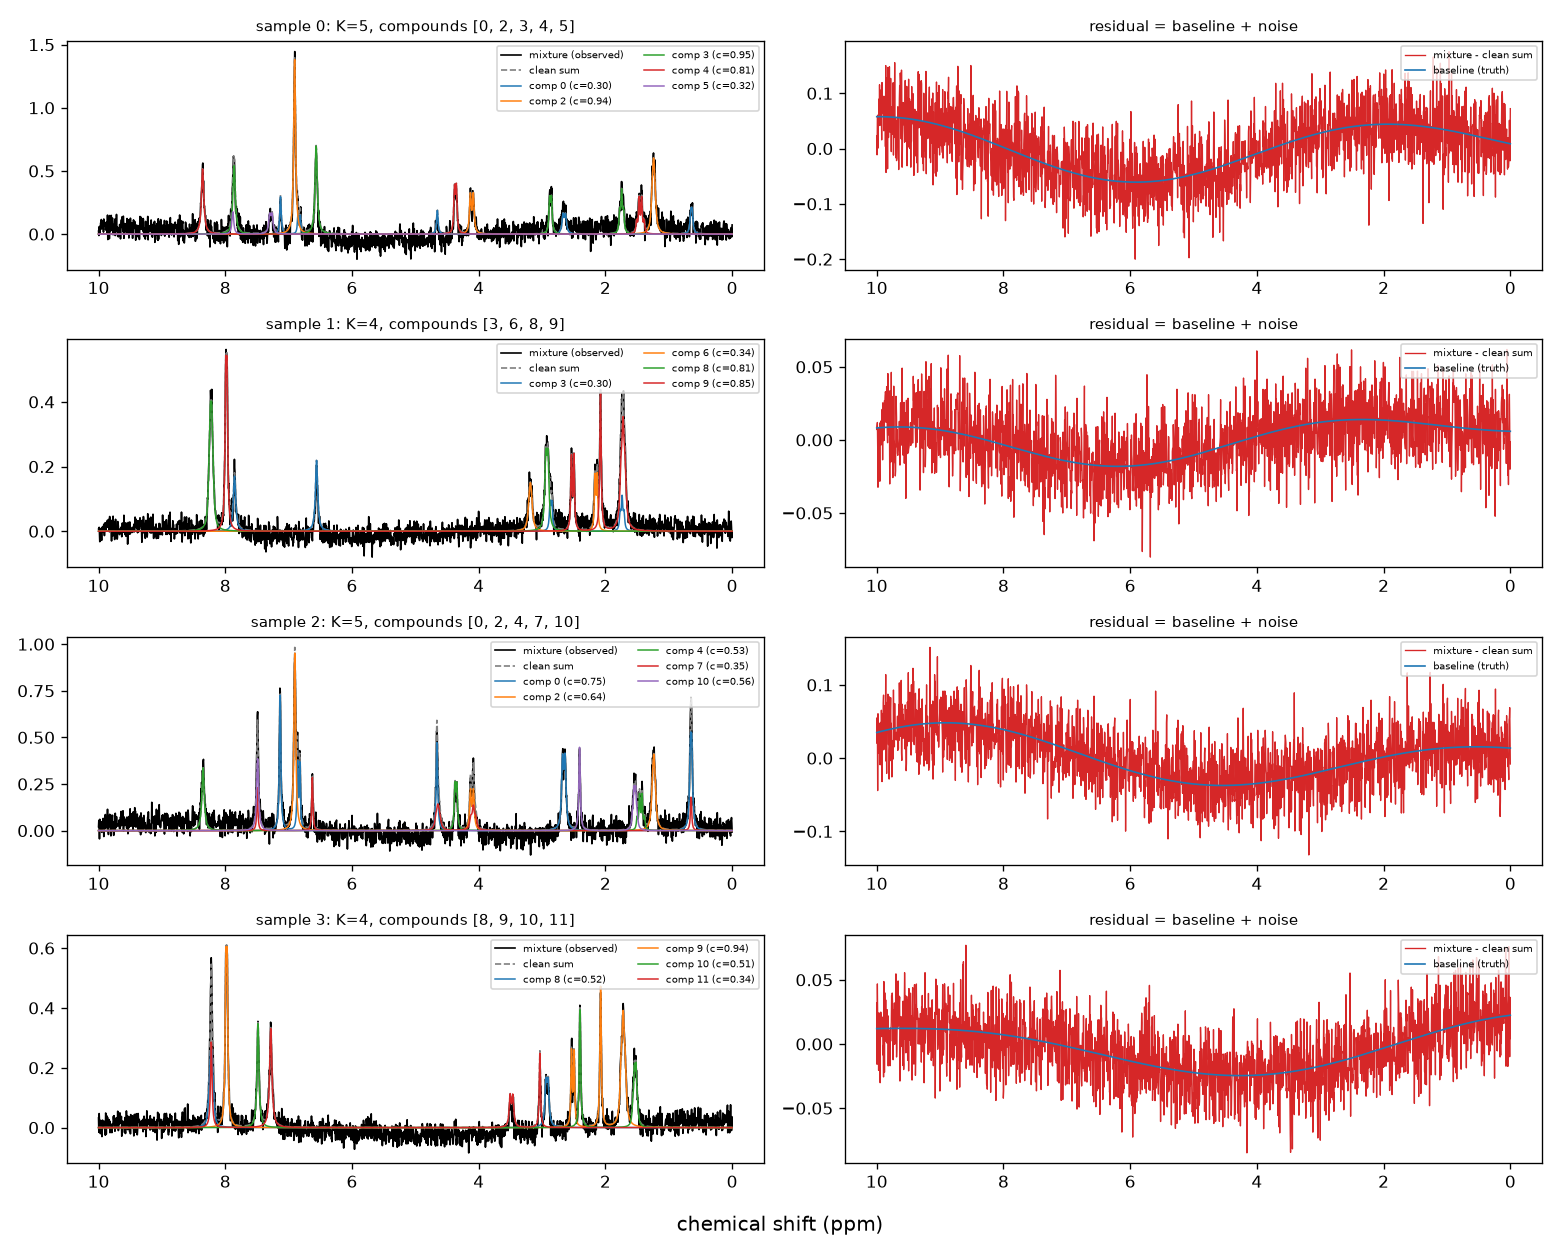
\includegraphics[width=0.82\textwidth]{mixtures.png}
  \caption{Generated mixtures (black) with the individual components summed into them.
  Ground truth is exact by construction, which is what makes disentanglement measurable.}
  \label{fig:mixtures}
\end{figure}

\paragraph{The difficulty knob.} A single scalar $d \in [0,1]$ interpolates three quantities
from an easy regime to a hard one: SNR from 40 to 6, maximum component count from 2 to 5, and
position jitter from 0.002 to 0.010~ppm. It drives Section~\ref{sec:robust}. It is a
\emph{bundle} of three knobs rather than a scalar measure of hardness, which matters when
reading the curves: because $k_{\max} = \mathrm{round}(\mathrm{lerp}(2,5,d))$ takes values
$2,3,4,4,5$ across the five sweep points, $d{=}0.50$ and $d{=}0.75$ share $k_{\max}{=}4$ and
differ only in noise and jitter.

\section{Model and input representation}

The model reads a spectrum as a sequence. One token per grid point is wasteful: attention
scales with the square of sequence length and most of a spectrum is empty baseline. A list of
picked peaks throws away the raw signal and the corruptions, and would not transfer to a
reconstruction objective. So I patch the signal as a vision transformer patches an
image~\cite{vit}. The 2048 points are cut into 64 non-overlapping patches of 32 points, each
linearly embedded to 128 dimensions by a strided convolution. A learned CLS token is
prepended, learned positional embeddings are added, and the sequence passes through four
pre-norm transformer encoder layers with four heads. The classifier reads CLS through a linear
layer to 12 presence logits. The model has $\approx$544k parameters and trains in under a
minute on a laptop GPU. The patch layout is deliberately the layout pretraining masks, so the
encoder is shared across every phase and its weights carry over unmodified.

\section{Masked pretraining}

Pretraining hides random spans and asks the model to fill them in. Masked patch embeddings are
replaced by a single learned mask token, the shared encoder runs, and a linear head predicts
raw values for every patch. The loss is mean squared error on masked patches only, so the
model gets no credit for copying what it can see. I mask contiguous spans rather than isolated
patches - half the patches, in spans of four ($\approx$128 points, wide enough to swallow a
whole peak). Single-patch masking is too easy, since a hidden point is interpolable from its
neighbors; spans force longer-range structure.

Pretraining uses 20{,}000 unlabeled mixtures from a stream disjoint from all labeled data.
Held-out reconstruction error falls from 0.0089 to 0.0038 over 20 epochs and is still
decreasing. The reconstructions (Figure~\ref{fig:recon}) are informative: in masked regions
the model places peaks close to where the hidden truth has them, and reconstructs a
\emph{denoised} version rather than the noisy measurement. That it recovers clean peak
structure from partial context, without labels, is the first evidence it learned something
about how these spectra are built. The objective's main flaw is a height bias: MSE under
partial information favors conservative guesses, so tall peaks are under-predicted and faint
ones can be missed.

\begin{figure}[t]
  \centering
  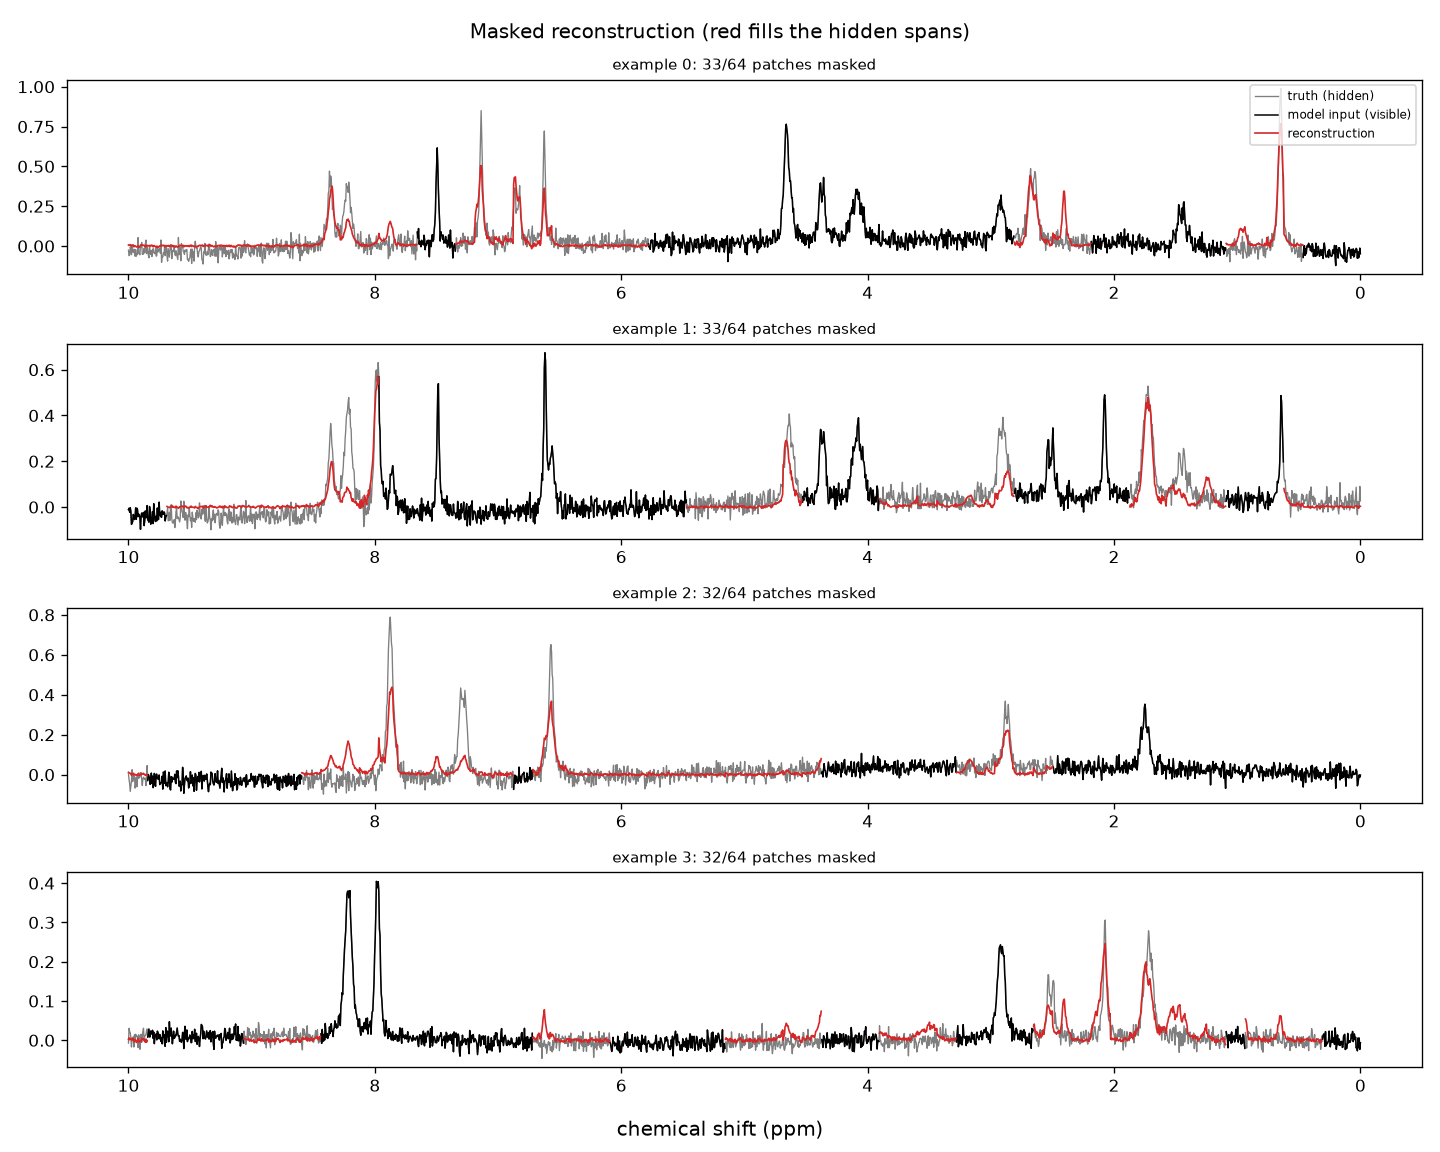
\includegraphics[width=0.78\textwidth]{pretrain_reconstructions.png}
  \caption{Masked reconstruction. Red fills the hidden spans; grey is the withheld truth.
  The model places peaks correctly and denoises rather than copying the measurement.}
  \label{fig:recon}
\end{figure}

\section{Experiments}

\subsection{From-scratch baseline}

Trained from scratch on presence classification with 4000 labels, the model reaches validation
macro-F1 0.997 and gets all 12 labels right on 97.8\% of samples, with no overfitting. That
number is high, and it is worth being honest about why: with a fixed library of distinct
fingerprints, presence detection is close to matched filtering, and a capable model saturates
it once labels are plentiful. This has a direct consequence for the study - pretraining
cannot improve on 0.997, so any benefit must appear where the baseline is weak: few labels, or
harder conditions.

\subsection{Fine-tuning: pretrained versus from-scratch}
\label{sec:finetune}

The headline comparison fine-tunes the full model at a range of label budgets, initializing
the encoder either randomly or from pretrained weights, holding everything else fixed: same
head init, same batch order, same optimizer, same 600-step budget, same seed. The only
variable is the encoder starting point. I report best validation macro-F1 over training,
averaged over three seeds.

\begin{table}[h]
\centering
\begin{tabular}{rccc}
\toprule
labeled examples & from scratch & pretrained & difference \\
\midrule
10   & $0.423 \pm 0.021$ & $0.453 \pm 0.051$ & $+0.030$ \\
40   & $0.711 \pm 0.021$ & $0.711 \pm 0.013$ & $+0.000$ \\
160  & $0.946 \pm 0.010$ & $0.954 \pm 0.005$ & $+0.008$ \\
640  & $0.994 \pm 0.001$ & $0.995 \pm 0.001$ & $+0.001$ \\
2560 & $0.998 \pm 0.001$ & $0.998 \pm 0.001$ & $-0.000$ \\
\bottomrule
\end{tabular}
\caption{Label efficiency on the default regime. The result is close to a null.}
\end{table}

Pretraining gives a small edge at the smallest budget, but $0.030$ at 10 labels is smaller
than its own standard deviation, so I do not read it as a real effect. Everywhere else the two
initializations are indistinguishable. \emph{Taken alone, this experiment says pretraining
does not help.} My working explanation was that full fine-tuning on an easy task lets the
from-scratch model reach the same solution, erasing any head start. The next experiment tests
that explanation directly.

\subsection{Linear probes on frozen features}
\label{sec:probes}

To separate representation quality from the effect of fine-tuning, I freeze each encoder and
train only a linear layer on its features. A linear probe is a sharp test: it cannot compute
structure that is absent, only read structure that is present. I compare a random untrained
encoder (the floor), the masked-pretrained encoder, and an encoder trained on 4000 presence
labels (a ceiling), on three targets: presence, component count $K$, and concentrations.
Features are mean-pooled over patch tokens - not the task-specific CLS, so no encoder is
privileged - and standardized.

\begin{table}[h]
\centering
\begin{tabular}{lccc}
\toprule
target & random & pretrained & supervised \\
\midrule
presence macro-F1 (2560 probe labels) & 0.729 & \textbf{0.872} & 0.998 \\
component-count accuracy              & 0.591 & \textbf{0.626} & 0.842 \\
concentration MAE (lower is better)   & 0.239 & \textbf{0.150} & 0.138 \\
\bottomrule
\end{tabular}
\caption{Frozen linear probes. Standard deviations are 0.001--0.013, so the gaps are real.}
\end{table}

The pretrained encoder beats the random one on every target at every budget. The concentration
result is the most convincing: an encoder that never saw a label decodes concentration almost
as well as one trained on labels (0.150 vs 0.138), and far better than random (0.239).
Presence is an oracle comparison for the supervised encoder, since it trained on presence;
concentration is the fair one, and it is where pretraining nearly matches supervision.

\subsection{Robustness: sweeping the difficulty knob}
\label{sec:robust}

Phases above run on one regime. Here I sweep $d$ and, at each point, pretrain a \emph{fresh}
encoder on unlabeled mixtures from that same difficulty. Reusing one encoder across the sweep
would confound two effects - the task getting harder, and the pretraining data no longer
matching the test data - and matched pretraining also mirrors the realistic setting: many
unlabeled spectra from your own instrument, few labels.

\begin{figure}[t]
  \centering
  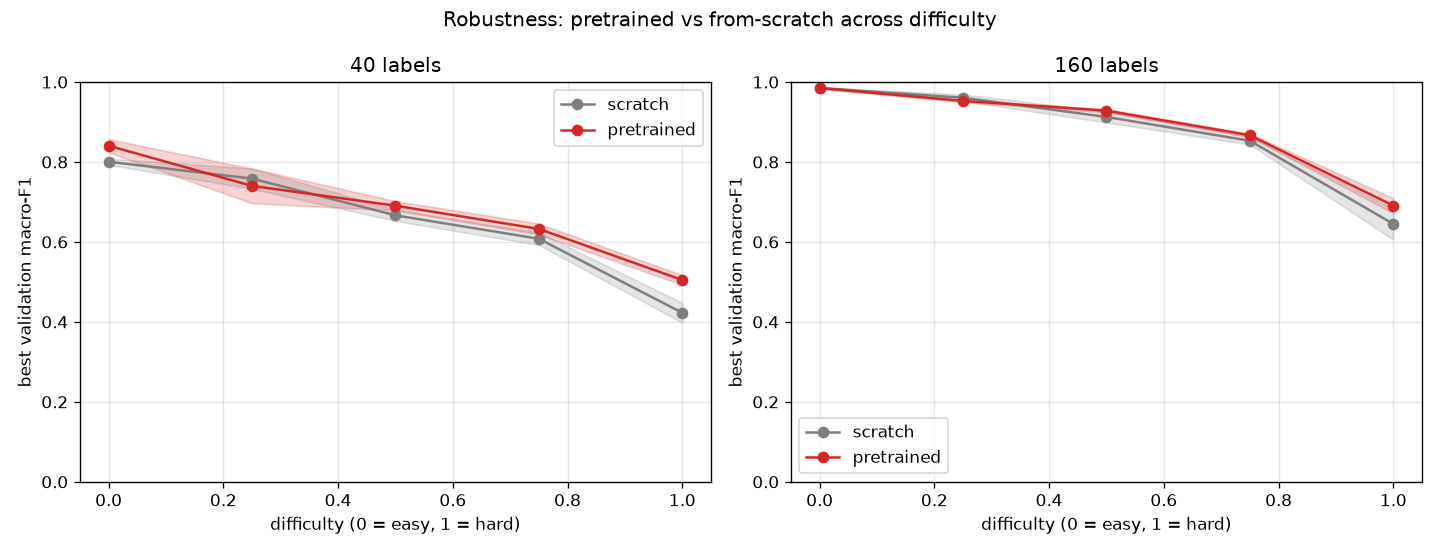
\includegraphics[width=\textwidth]{robustness_finetune.png}
  \caption{Fine-tuning across difficulty. The pretraining gain is largest at the hard end at
  the smallest budget, but the effect is small next to the overall degradation.}
  \label{fig:robustft}
\end{figure}

The standing prediction was that the null gap of Section~\ref{sec:finetune} reappears once the
task is hard enough that a from-scratch model cannot catch up in a fixed budget. It is
\emph{partially} supported, and only at the smallest budget. Because scratch and pretrained
runs share a seed, the honest statistic is the paired per-seed gain:

\begin{table}[h]
\centering
\begin{tabular}{lcc}
\toprule
difficulty $d$ & gain at 40 labels & gain at 160 labels \\
\midrule
0.00 & $+0.040$ (3/3 seeds $+$) & $-0.000$ (mixed) \\
0.25 & $-0.018$ (mixed)          & $-0.008$ \\
0.50 & $+0.024$ (3/3 seeds $+$)  & $+0.016$ (mixed) \\
0.75 & $+0.025$ (3/3 seeds $+$)  & $+0.014$ \\
1.00 & $\mathbf{+0.082}$ (3/3 seeds $+$) & $+0.046$ (mixed) \\
\bottomrule
\end{tabular}
\caption{Paired per-seed fine-tuning gains (pretrained minus scratch).}
\end{table}

The one solid claim is $+0.082$ at $d{=}1.00$ with 40 labels: all three seeds positive, about
four times the seed spread. I resist the tidier story for three reasons. The curve is not
monotone - $d{=}0.00$ also shows a consistent $+0.040$, so ``no gap when easy'' is false
here. The $d{=}0.25$ dip is mixed-sign and within noise. And the $+0.046$ at 160 labels and
$d{=}1.00$ is driven by a single seed ($+0.116$, with another at $-0.014$, standard deviation
$0.054 >$ mean); I do not treat it as a result.

\begin{figure}[t]
  \centering
  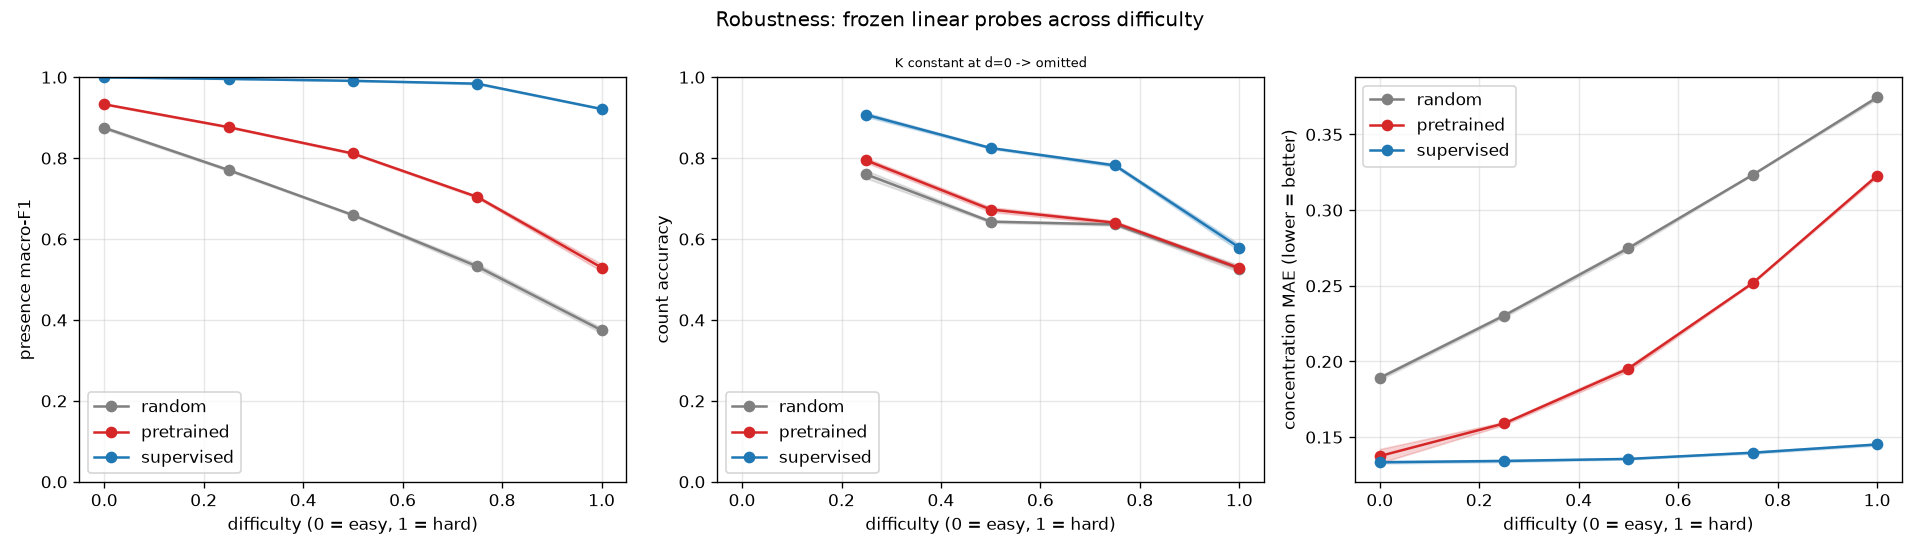
\includegraphics[width=\textwidth]{robustness_probe.png}
  \caption{Frozen probes across difficulty. The pretrained-over-random advantage widens with
  difficulty, but the supervised encoder degrades far more gracefully than either.
  The count probe is omitted at $d{=}0$, where $K$ is constant and the metric is degenerate.}
  \label{fig:robustprobe}
\end{figure}

The probe arm is more interesting. The pretrained encoder beats random at every difficulty,
with the advantage widening from $+0.058$ to $+0.172$ at $d{=}0.75$ before narrowing as
everything collapses. But the asymmetry at the hard end is the real result:

\begin{table}[h]
\centering
\begin{tabular}{lccc}
\toprule
$d$ & random & pretrained & supervised \\
\midrule
0.00 & 0.875 & 0.933 & 1.000 \\
0.25 & 0.771 & 0.877 & 0.996 \\
0.50 & 0.659 & 0.811 & 0.991 \\
0.75 & 0.532 & 0.704 & 0.984 \\
1.00 & 0.374 & 0.529 & \textbf{0.921} \\
\bottomrule
\end{tabular}
\caption{Presence macro-F1 on frozen features across difficulty.}
\end{table}

At $d{=}1.00$ the supervised encoder still reaches 0.921 presence macro-F1, and its
concentration MAE is nearly flat across the whole sweep (0.133 to 0.145), while the pretrained
encoder falls to 0.529 and 0.323. \emph{The information is still there and still linearly
decodable} - supervision proves it. The task is not intrinsically impossible at SNR 6. It is
the pretext task that stops capturing the structure.

\paragraph{A methodological artifact worth naming.} At $d{=}0$ the knob pins $k_{\max}$ to
$k_{\min}{=}2$, so every mixture has exactly $K{=}2$, the count probe has a single class, and
\emph{every} encoder scores 1.000 - including the random control. That is an artifact of the
knob, not a result, and it is reported as ``n/a'' rather than as a perfect score.

\subsection{Which part breaks: a pretext-target ablation}
\label{sec:ablation}

Section~\ref{sec:robust} leaves a specific hypothesis, which I recorded before testing it: if
the supervised encoder reads compound identity at SNR 6 but the pretrained one cannot, perhaps
the problem is \emph{what the pretext predicts}. At SNR 6 the observed signal is largely noise,
and noise is precisely the unpredictable part, so the masked-MSE gradient may be spent
modelling noise rather than structure. If true, the fix is to change the target.

I therefore change only the target, holding masking, architecture, budget, seeds, and probe
fixed. The \texttt{raw} arm reconstructs the observed noisy signal (the original pretext); the
\texttt{clean} arm reconstructs the noise-free component sum. One honesty note governs the
reading: the clean signal is ground truth no real unlabeled setting would provide, so the clean
arm is \textbf{not} self-supervised. It is an oracle, deliberately - a diagnostic that upper
bounds what any better target could buy. The control behaves correctly: at $d{=}0$, where
SNR is 40 and there is almost no noise to remove, the arms are indistinguishable (0.933 vs
0.936), which licenses reading any hard-end difference as being about noise.

\begin{table}[h]
\centering
\begin{tabular}{lccccc}
\toprule
$d$ & random & raw & clean & supervised & gap recovered by clean \\
\midrule
0.00 & 0.875 & 0.933 & 0.936 & 1.000 & $+4\%$ \\
0.50 & 0.659 & 0.811 & 0.815 & 0.991 & $+2\%$ \\
0.75 & 0.532 & 0.704 & 0.720 & 0.984 & $+6\%$ \\
1.00 & 0.374 & 0.529 & \textbf{0.539} & 0.921 & $\mathbf{+2\%}$ \\
\bottomrule
\end{tabular}
\caption{Presence macro-F1 on frozen features. Swapping in a perfect target changes almost
nothing: the hypothesis is refuted.}
\end{table}

\begin{figure}[t]
  \centering
  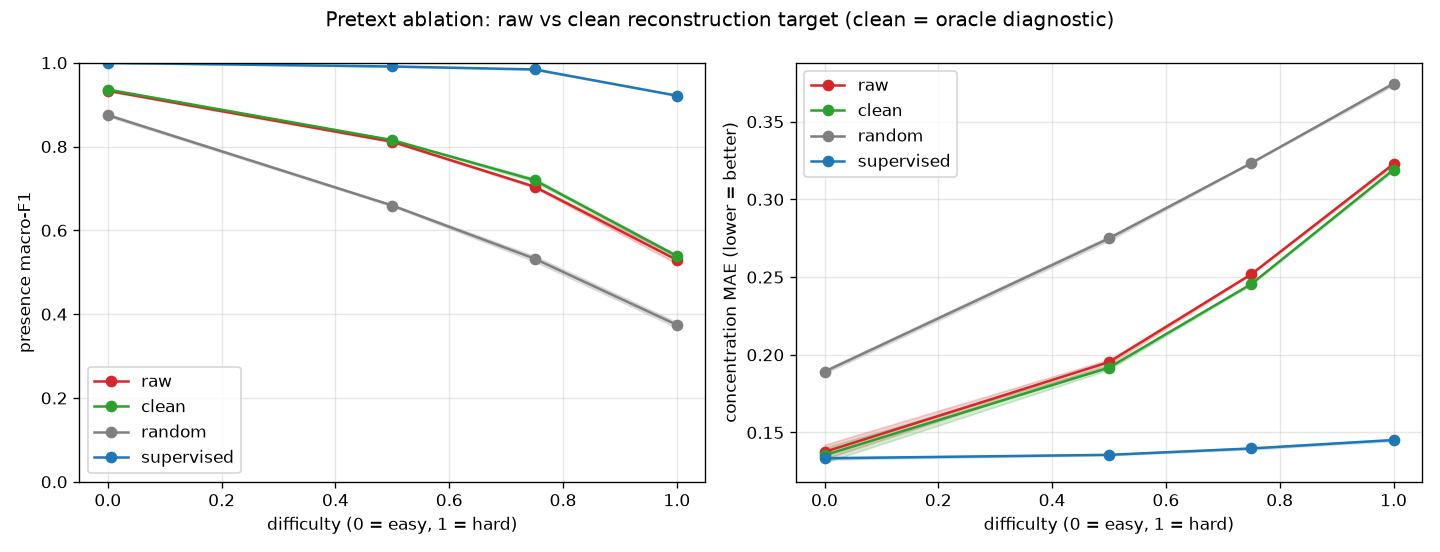
\includegraphics[width=\textwidth]{pretext_ablation.png}
  \caption{Raw (red) and clean (green) reconstruction targets produce near-identical
  representations at every difficulty, both far below supervised (blue).}
  \label{fig:ablation}
\end{figure}

\textbf{The hypothesis is wrong.} Handed a perfect noise-free target at the hard end, the
pretext gains $0.010$ macro-F1 - 2\% of the $0.392$ gap to supervised. Standard deviations
are $0.001$--$0.009$, so this is a real non-effect, and concentration error agrees ($0.323 \to
0.319$). Noise in the reconstruction target is not why masked pretraining collapses at low SNR.

This is worth its cost for two reasons. It kills the obvious follow-up: a Noise2Noise-style
target~\cite{noise2noise} was the natural genuinely-self-supervised version of this fix, and if
the \emph{oracle} buys nothing, no self-supervised approximation to it will do better. And it
sharpens the open question. My leading candidate explanation - untested - is that masked
reconstruction is solvable \emph{locally}: filling a hidden span only requires continuing the
peak shapes suggested by neighbouring context, never knowing which compound produced them. The
objective would then never reward identity, while supervised training optimizes it directly,
which would explain why supervision holds at 0.921. A duller possibility must be excluded
first, because it is a measurement artifact rather than a claim about learning: the probe reads
mean-pooled patch tokens, so information held nonlinearly or concentrated in CLS would be
invisible to it.

One result survives the ablation intact, and the two should be held together: the fine-tuning
gain at the hard end ($+0.082$ at 40 labels, all seeds agreeing) is untouched. Pretraining
still helps \emph{fine-tuning} where labels are scarce and the task is hard, even though its
\emph{frozen} features are weak there.

\section{Discussion}

The experiments only make sense together. Fine-tuning says final accuracy is the same whether
or not you pretrain. Probing says the pretrained representation is much better organized for
the properties that define a mixture. Both are true, and the tension is the finding. When the
whole model is free to move and the task is easy, the from-scratch model learns whatever
features it needs and reaches the same place, so a head start does not change the destination.
When the encoder is frozen, the head start is all there is, and pretrained features win
clearly.

This answers the question the project was built around - whether the model learns real
structure or memorizes a mapping. A linear probe cannot read out component count or
concentration unless the representation has arranged that information simply, and the
pretrained encoder arranges it well enough that a linear readout of concentration nearly
matches a supervised encoder. That is structure, not surface memorization. It also reframes
the fine-tuning null as a statement about the task and protocol rather than about the
representation.

The difficulty sweep then adds a caution that I did not expect and would not have found on the
easy regime alone. It is tempting to read ``self-supervised pretraining learns physical
structure'' as a general claim. It is not: the structure it learns is contingent on the
pretext objective remaining informative, and a raw-reconstruction objective stops being
informative exactly where you would most want help - in the low-SNR regime where labels are
expensive and a good prior matters most.

\section{Limitations}

The data is synthetic and, at default settings, not hard: peaks are distinct, noise is
moderate, mixtures hold at most five components, and the supervised task saturates quickly.
The model is small by design. The reconstruction objective has a height bias that
under-predicts tall peaks. The supervised encoder is an oracle ceiling for presence, so the
fair comparison is concentration. The random encoder is a single draw rather than an average
over initializations. In the difficulty sweep, one encoder per difficulty is shared across
seeds, so the error bars capture fine-tuning and probe variance but \emph{not}
pretraining-run variance - a real gap, since a single unlucky pretraining run would be
invisible to those bars. The difficulty knob bundles three quantities, so the $x$-axis is not
a clean scalar. And the whole study is one architecture at one size; none of these results
speak to what a larger model would do.

\section{Future work}

Section~\ref{sec:ablation} redirects this section, which is the most useful thing it did. A
noise-robust objective is \emph{ruled out}, not indicated: if the oracle target recovers 2\% of
the gap, no self-supervised approximation to it will do better.

The real next step is to separate the two live explanations, cheapest first. Re-probe the
existing encoders with CLS pooling and with a small MLP probe: this needs no retraining and
determines whether the collapse is a property of the representation or of how I read it. Only
if the information is genuinely absent does the interesting explanation stand - that masked
reconstruction is solvable by local continuation and never requires compound identity. That
explanation predicts a concrete fix: a pretext that \emph{cannot} be solved locally, such as
masking contiguous regions far wider than a multiplet, or masking one compound's peaks wherever
they occur across the spectrum, forcing global integration rather than interpolation.
Contrastive objectives over mixtures sharing components apply the same pressure.

Beyond that: swapping the parametric library for real single-compound spectra from
nmrshiftdb2; a separation head that reconstructs individual component signals rather than
classifying presence; an attention analysis checking whether attention concentrates on peak
regions rather than empty baseline; and more seeds, which the paired analysis shows would
sharpen several of the marginal claims here.

\section{Reproducibility}

The project is Python and PyTorch with a short dependency list. Configuration lives in YAML
files mapped onto typed dataclasses, so there are no hard-coded constants, and every entry
point seeds all random number generators from its config. A 46-test suite covers the
reconstruction identity and other generator invariants, seeding determinism, model shapes,
metrics, masking, weight transfer, the difficulty knob, and the probes. \texttt{python
scripts/run\_all.py} reruns every experiment in this paper in order and regenerates every
figure. Development ran on Apple Silicon (MPS); the same code runs on a single CUDA GPU.
Code: \url{https://github.com/tanmayhinge/spectral-disentangling}.

\begin{thebibliography}{9}
\bibitem{bert} J. Devlin, M.-W. Chang, K. Lee, K. Toutanova.
  \emph{BERT: Pre-training of Deep Bidirectional Transformers for Language Understanding.}
  NAACL, 2019.
\bibitem{mae} K. He, X. Chen, S. Xie, Y. Li, P. Doll\'ar, R. Girshick.
  \emph{Masked Autoencoders Are Scalable Vision Learners.} CVPR, 2022.
\bibitem{vit} A. Dosovitskiy et al.
  \emph{An Image is Worth 16x16 Words: Transformers for Image Recognition at Scale.}
  ICLR, 2021.
\bibitem{noise2noise} J. Lehtinen et al.
  \emph{Noise2Noise: Learning Image Restoration without Clean Data.} ICML, 2018.
\end{thebibliography}

\end{document}
